\documentclass[11pt]{exam}

\usepackage{amsmath, amssymb, multicol}
\usepackage{graphicx}
\usepackage{textcomp}
\usepackage{chessboard}

\def\d{\displaystyle}
\def\b{\mathbf}
\def\R{\mathbf{R}}
\def\Z{\mathbf{Z}}
\def\st{~:~}
\def\bar{\overline}
\def\inv{^{-1}}

\def\v{circle (3pt)}


%\pointname{pts}
\pointsinmargin
\marginpointname{pts}
\addpoints
\pagestyle{head}
%\printanswers

\firstpageheader{Math 228}{\bf From Dots to Sequences}{Friday, Feb 20}


\begin{document}

%space for name
%\noindent {\large\bf Name:} \underline{\hspace{2.5in}}
%\vskip 1em

\subsection*{Activity 1: Dots}

For the patterns of dots below, draw the next pattern in the sequence.  Then give a recursive definition and a closed formula for the number of dots in the $n$th pattern. 


  \begin{multicols}{4}
  \begin{center}
  
\begin{tikzpicture}
  \draw[fill = black] (0,0) \v;
  \end{tikzpicture}
  
  $n = 0$
  \end{center}
  
  \columnbreak
    \begin{center}
    
\begin{tikzpicture}
    \draw[fill = black] (0,0) \v (.3, .3) \v (-.3,-.3) \v (-.3, .3) \v (.3,-.3) \v;
    \end{tikzpicture}
    
    $n = 1$
    \end{center}
    
    \columnbreak
    
    \begin{center}
    
\begin{tikzpicture}
    \draw[fill = black] (0,0) \v (.3, .3) \v (-.3,-.3) \v (-.3, .3) \v (.3,-.3) \v (.6, .6) \v (-.6,-.6) \v (-.6, .6) \v (.6,-.6) \v;
    \end{tikzpicture}
    
    $n = 2$
    \end{center}
    
    \columnbreak

	~
  \end{multicols}
  
\vfill


  \begin{multicols}{4}
  \begin{center}
  
\begin{tikzpicture}
  \draw[fill = black] (0,0) \v (0,2) \v;
  \end{tikzpicture}
  
  $n = 0$
  \end{center}
  
  \columnbreak
    \begin{center}
    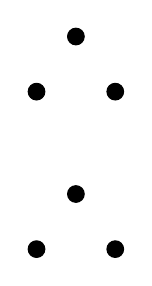
\begin{tikzpicture}
    \draw[fill = black] (-.5,0) \v (.5, 0) \v (0, .7) \v (-.5,2) \v (.5, 2) \v (0,2.7) \v;
    \end{tikzpicture}
    
    $n = 1$
    \end{center}
    
    \columnbreak
    
    \begin{center}
    
\begin{tikzpicture}
    \draw[fill = black] (-.7,0) \v (-.3,0) \v (-.5,.35) \v 
    	(.3, 0) \v (.7,0) \v (.5, .35) \v
    	(-.2, .7) \v (.2, .7) \v (0, 1.05) \v 
    	(-.7, 2) \v (-.3, 2) \v (-.5,2.35) \v 
    	(.3, 2) \v (.7, 2) \v (.5, 2.35) \v 
    	(-.2,2.7) \v (.2, 2.7) \v (0,3.05) \v;
    \end{tikzpicture}
    
    $n = 2$
    \end{center}
    
    \columnbreak
    \vskip 1in
    
    ~
  \end{multicols}

\vfill

  \begin{multicols}{5}
  \begin{center}
  
\begin{tikzpicture}
  \draw[fill = black] (0,0) \v;
  \end{tikzpicture}
  
  $n = 1$
  \end{center}
  
  \columnbreak
    \begin{center}
    
\begin{tikzpicture}
    \draw[fill = black] (0,0) \v (.5, 0) \v (.25,.4) \v;
    \end{tikzpicture}
    
    $n = 2$
    \end{center}
    
    \columnbreak
    
    \begin{center}
    
\begin{tikzpicture}
    \draw[fill = black] (0,0) \v (.5, 0) \v (.25,.4) \v (1,0) \v (.75,.4) \v (.5, .8) \v;
    \end{tikzpicture}
    
    $n = 3$
    \end{center}
    
    \columnbreak
    
        \begin{center}
        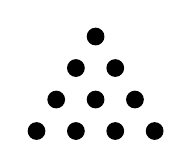
\begin{tikzpicture}
        \draw[fill = black] (0,0) \v (.5, 0) \v (.25,.4) \v (1,0) \v (.75,.4) \v (.5, .8) \v (1.5, 0) \v (1.25, .4) \v (1, .8) \v (.75, 1.2) \v;
        \end{tikzpicture}
        
        $n = 4$
        \end{center}
        
        \columnbreak
     
     ~
  \end{multicols}
\vfill

\newpage

\subsection*{Activity 2: Sequences}

For each sequence of numbers, guess the next term in  the sequence.  Then find a recursive definition and closed formula for the $n$th term of the sequence.  Assume the first term given is $a_0$.

\begin{itemize}
\item 3, 6, 12, 24, \ldots
\vfill
\item 2, 5, 8, 11, \ldots
\vfill
\item 4, 12, 20, 28, \ldots
\vfill
\item 4, 12, 36, 108, \ldots
\vfill
\item 2, 5, 10, 17, 26, \ldots 
\vfill
\end{itemize}



\end{document}


